\documentclass[twocolumn,12pt]{article}
\usepackage[a4paper,portrait,margin=0.5in]{geometry}

\usepackage{amsmath}
\usepackage{amssymb}
\usepackage{amsthm}
\usepackage[toc,page]{appendix}
\usepackage{graphicx}
\usepackage{caption}
\usepackage{placeins}
\usepackage{float}
\usepackage{tabularx}
\usepackage{array,booktabs}
\usepackage{bm}
\usepackage{bbm}
\usepackage{siunitx}
\usepackage[skip=0pt]{caption}
\usepackage{sectsty}

\sectionfont{\fontsize{12}{15}\selectfont}
\usepackage{titling}

\setlength{\droptitle}{-2cm}

\newcommand{\czt}{\tilde{c}_2}
\newcommand{\cdt}{\tilde{c}_3}
\newcommand{\DKL}{D_\mrm{KL}}
\newcommand{\Eden}{E^\mrm d}
\newcommand{\Esom}{E^\mrm s}
\newcommand{\ipsum}{{\bf IPSUM}}
\newcommand{\lb}{\left}
\newcommand{\lorem}{{\bf LOREM}}
\newcommand{\mb}{\mathbf}
\newcommand{\mrm}{\mathrm}
\newcommand{\mV}{\milli\volt}
\newcommand{\N}{\mathbb N}
\newcommand{\R}{\mathbb R}
\newcommand{\rb}{\right}
\newcommand{\Spre}{\Sigma_{\mrm{usp}}}
\newcommand{\todoin}[1]{\todo[inline]{#1}}
\newcommand{\todosolved}[1]{\todo[inline, color=green]{#1}}
\newcommand{\un}{\mb{1}}
\newcommand{\wden}{w^\mrm d}
\newcommand{\wsom}{w^\mrm s}
\newcommand{\xeps}{\mathbf x^{\epsilon}}

\begin{document}
\setlength{\abovedisplayskip}{3pt}
\setlength{\belowdisplayskip}{3pt}
\title{Natural Gradient Learning for Spiking Neurons \vspace*{-3cm}}
\date{}
\maketitle

\section*{Abstract}
\vspace*{-0.3cm}
Due to their simplicity and success in machine learning, gradient-based learning rules represent a popular choice for synaptic plasticity models. While they have been linked to biological plasticity experiments, it is often ignored that their predictions generally depend on a specific representation of the synaptic strength. In a neuron, the impact of a synapse can be described simultaneously by the state of many physical quantities inside the cell. Which one we choose to derive a gradient descent learning rule can have a remarkable effect in terms of model prediction. This is dissatisfying both from the viewpoint of fast learning, as well as from a conceptual angle. Plasticity should strive to adjust the neuron's output firing in an optimal fashion, rather than an internal parameter, but classical gradient rules fail to accomplish this goal. Natural gradient descent provides a solution to both problems by following the gradient on the manifold of the neuron's firing distributions, combining the intuition of gradient descent with the elegance of an output change that is invariant under a change of representation. While the computational advantages of natural gradient are well-studied in ANNs, its predictive power as a model for in-vivo synaptic plasticity has not been assessed. We demonstrate that it exhibits faster convergence compared to classical gradient learning in a network of spiking neurons. Furthermore, our approach provides a unified framework for both homo- and heterosynaptic plasticity and  predicts plasticity phenomena such as learning rate scaling in distal dendrites.
\vspace*{-0.7cm}
\section*{Plasticity Rule}
\vspace*{-0.3cm}
We explore the biological predictions and learning performance of natural gradient descent learning (Amari 1998, Ollivier 2015) in the context of a supervised learning task with Poisson spiking neurons (see Fig 1A). Receiving Poisson spike trains from afferent nerve cells, a neuron had to respond by firing spikes according to a target distribution, delivered via spikes from a teacher neuron. The student neuron's firing rate was a given as a nonlinear function $\phi$ of the somatic membrane potential $V=\sum_i w_i x_i^{\epsilon}$. Here  $x_i^{\epsilon}$ denote unweighted synaptic potentials (USP), evoked by presynaptic input, which were weighted by the somatic amplitudes $w_i$. We obtained the natural gradient descent learning rule as 
\begin{eqnarray}
\label{Results_Natural_Gradient}
\dot{\mb w} =\eta \ \gamma_{\mrm s} \lb(Y^*-\phi(V)\rb) \frac{\phi'(V)}{\phi(V)}\lb(\frac{c_{\epsilon}\xeps}{\mb r}-\gamma_{\mrm u}+\gamma_{\mrm w}{\mb w}\rb),
\end{eqnarray} 
where $Y^*$ denotes the teacher spiking. While the coefficients $\gamma_{\mrm s},\gamma_{\mrm u},\gamma_{\mrm w}$ are in general functions of the membrane potential, the total input, and their first and second moments, empirical evidence demonstrates that in many cases, they can be well approximated by simpler quantities easier accessible to the synapse.
\vspace*{-0.7cm} 
\section*{Biological Predictions}
\vspace*{-0.3cm}
Just as classical gradient rules, natural gradient plasticity follows the postsynaptic error (Eq 1), and its product with the USPs adjusts synapses that have recently been active. However, unlike for classical gradient learning, this homosynaptic weight update is complemented by both a uniform as as well as a weight-proportional heterosynaptic contribution. This is in line with experimental findings (Lynch 1977, Chistiakova 2009), as well as with computational studies that list heterosynaptic plasticity as a necessary component of stable learning (Zenke 2017). Qualitatively similar to experimental data (Lynch 1977, Royer \& Paré 2003), we found that under certain conditions, changes at unstimulated synapses exhibited an opposite sign compared to the plasticity at stimulated synapses, thereby keeping the neuron within its operational range.\\
Moreover, our learning rule includes a synapse-specific scaling of the homosynaptic contribution by the input rate, similar to the rescaling observed in a Bayesian plasticity framework (Aitchison 2014). Moreover, simulations revealed that under a simple stimulation protocol, the effective learning rate of our rule was inversely related to the USP variance. Additionally it is also subject to distance dependent scaling, which can be observed whern expressing the weight update directly in terms of EPSP amplitudes in the dendritic tree, rather than their somatic counterparts.
 Since synaptic changes are attenuated on their way to the soma, in order to evoke the same effect in terms of adapting the neuron's firing behavior, changes at distal synapses must be increased compared to plasticity at proximal synapses with a similar impact on output firing, conceptually reminding of the dendritic democracy concept (Häusser 2001).\\
 Our learning rule provides a consistent plasticity framework that combines fast learning together with multiple experimentally testable predictions, including a unified framework for both homo-and heterosynaptic changes.
 \begin{figure*}
\center
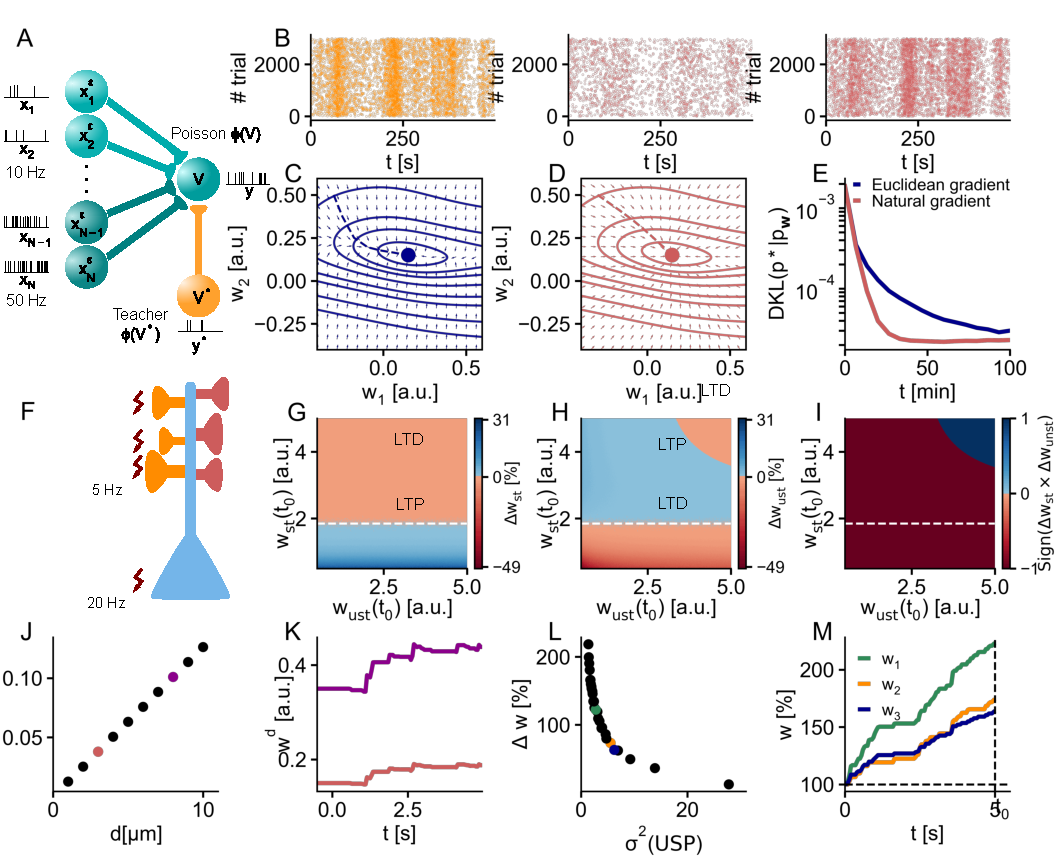
\includegraphics[width= .9\textwidth]{Figure_Cosyne2}
\caption{{\bf (A)} Learning task.{\bf(B-D)} Spike trains for teacher {\bf(B)}, and for student neuron before learning {\bf(C)} and after learning with the natural gradient rule {\bf(D)}. {\bf{(E-G)}} Contour lines of the $\DKL$ between output and target distribution and normalized vector plots for standard gradient vectors{\bf(E)} and natural gradient vectors {\bf(F)} together with weight path during learning. The classical gradient descent learning rule follows the contour lines of the error function, whereas the natural gradient rule updates synapses in direction of the target.%
{\bf(G)} Learning curves for natural and Euclidean descent learning. The natural gradient shows faster learning compared to the classical error learning rule. %
{\bf(H)-(K)} Direction of homo- and heterosynaptic plasticity in a simple experiment with variable excitatory input and tonic inhibition. We stimulated \num{5} out of ten afferents providing excitatory Poisson input at to a neuron, while simultaneously delivering tonic inhibition and a teacher spike train. We investigated the direction of synaptic changes at stimulated and unstimulated synapses as a function of the initial weights.{\bf (I)} Weight change of stimulated weights. While varying the size of the unstimulated weights had no effect, increasing the initial weight of the simulated synapses resulted in a change from potentation to depression. {\bf (J)} Weight change of the unstimulated weights. Heterosynaptic plasticity decreased the unstimulated weights in regions where the stimulated weights underwent LTP. Increasing the size of initial stimulated weights resulted in a change to potentiation at the same point where homosynaptic LTP turned into LTD. Further increase of either unstimulated or stimulated weights resulted eventually lead to depression of the unstimulated synapses. {\bf(K)} Example traces of absolute EPSP amplitude change at the dendrite, for a distal (purple) and a proximal synapse (red) with the same impact on output firing.{\bf(L)} Absolute dendritic amplitude change as a function of distance from soma is linearly increasing. The synaptic weight traces in {\bf(M)} show a higher weight change for low variance input compared to high USP variance scenarios.{\bf(N)} Synaptic weight change on the interval as a function of USP variance.}
\end{figure*}

\end{document}